\chapter{Research Design: Method, Questions, and Requirements}
This section defined how the study is designed and how it will be evaluated. We first outline the method used and state the research questions that guide our work. We then set the scope of work, keeping the focus on a modular classification pipeline with embedded continual learning for small teams with constrained resources. An industry use case is then introduced to ground the blueprint in a realistic scenario , which can evaluate our work.
\smallbreak


Next we derive the general requirements from the problem statement and the use case and explain how they shape our artifact. These requirements are use-case agnostic so the blueprint remains reusable. In later chapters , we will apply the requirements to the news-classification scenario and assess the blueprint.

\section{Methodology}
This study uses Design Science Research (DSR) , supported by a targeted literature review. The review will provide us with practical evidence of knowledge from data engineering , ML Ops, Text Classification and continuous learning. From these literature we will then derive requirements and design principles needed for a modular classification pipeline. Following the DSR cycle, we identify the problem and goals , design the artifact and evaluate it on a realistic industry related use case.
The methodological flow is shown in Figure~\ref{fig:dsr-loop}
The targeted literature review is based on searches of Google Scholar , springer and Research gate as primary sources, which includes practice oriented ETL and ML pipelines, continuous learning, modularity and classification studies. This review excludes pure algorithmic proposals and derives requirements from documented challenges from the listed topics.

\begin{figure}[htbp]
    \centering
    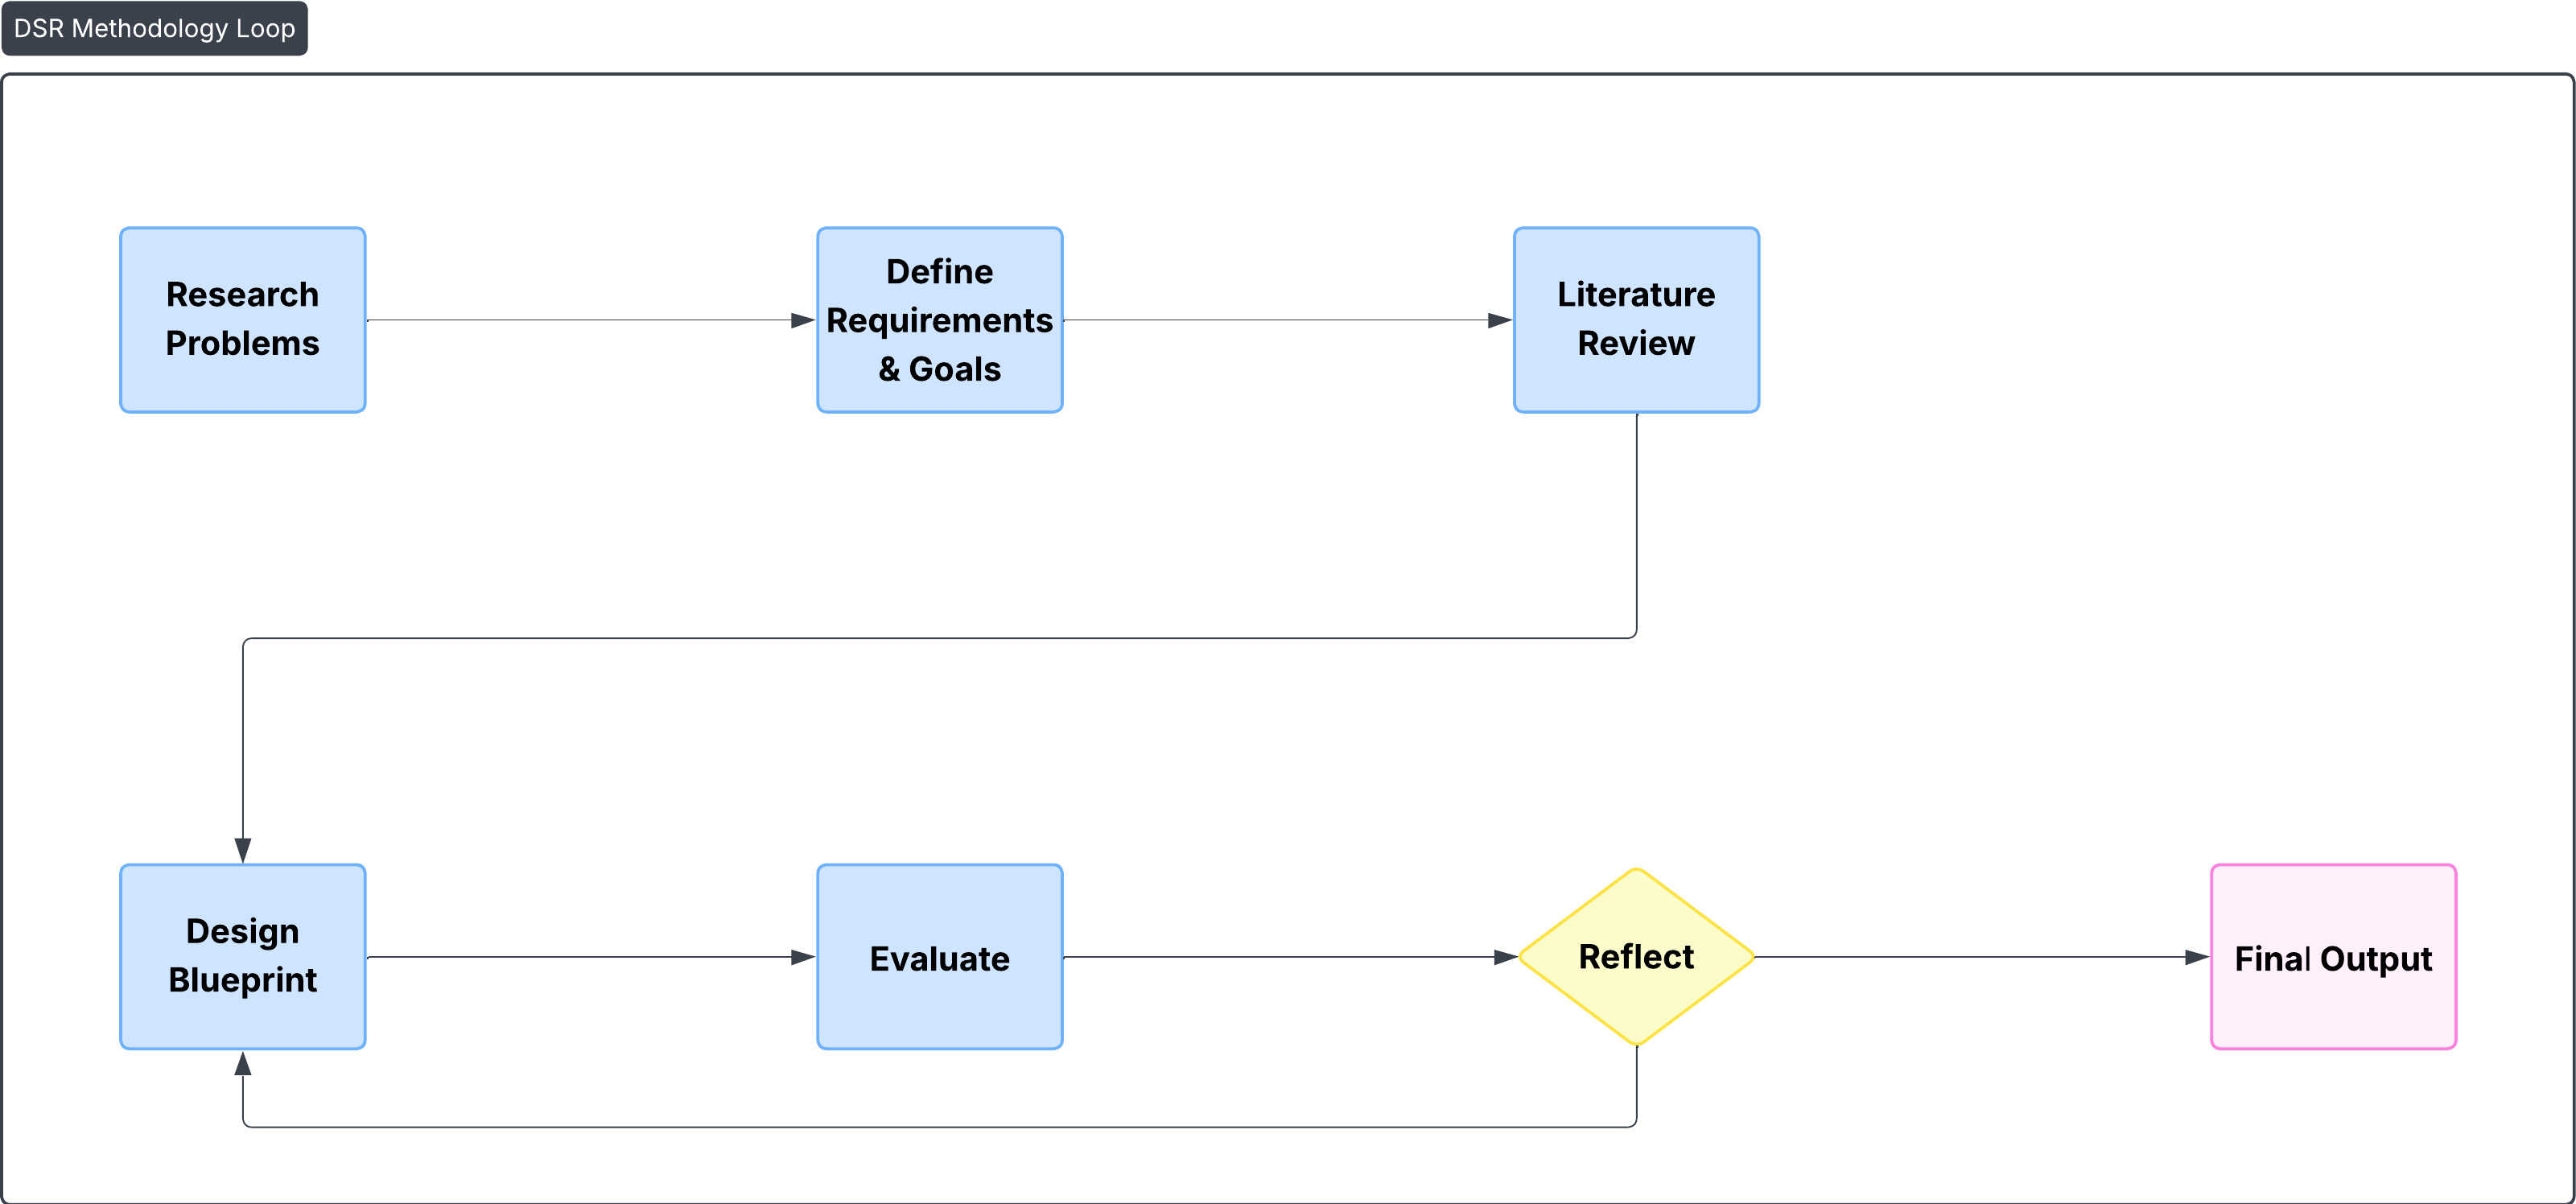
\includegraphics[width=\linewidth]{gfx/examples/dsr_loop.jpeg}
    \caption{Methodology: Design Science Research (DSR)}
    \label{fig:dsr-loop}
\end{figure}


\section{Problem Statement and Research Questions}
Organizations who want to build a ML classification solution, often lack the ability to develop and develop it. Success depends on the resources they allocate , which are frequently scarce, fragmented or poorly coordinated \cite{duda:2024}. Without a clear view on which resources matter the most , firms often misallocate effort and usually end up with costly , hard to reverse implementations.
When organizations finally move to implementation without enough upfront research , it is highly likely some unforeseen challenges might occur \cite{arpteg:2018}. During our literature review, we identified core challenges that recur across data and ML pipeline projects. To address them in a clear way , we are organizing the problems into two groups :

% --- Table 1: Foundational pipeline design ---
\begin{table}[htbp]
    \centering
    \begin{tabularx}{\linewidth}{@{}lX@{}}
        \toprule
        \textbf{\#} & \textbf{Problems in foundational pipeline design}                                                                                                   \\
        \midrule
        1           & Tight coupling : Updates in one component, causes a ripple effect that might break the whole system \cite{modi:2023}                                \\
        2           & Data Quality \& Governance: Inconsistent schemas and incorrectly defined data types lead to weak pipelines and unreliable models. \cite{foidl:2024} \\
        3           & Complexity: Modern MLOps tools are complex and costly for small companies. \cite{eken:2025}                                                         \\
        \bottomrule
    \end{tabularx}
    \caption{Problems in foundational pipeline design}
    \label{tab:problems_foundational}
\end{table}

% --- Table 2: Model lifecycle ---
\begin{table}[htbp]
    \centering
    \begin{tabularx}{\linewidth}{@{}lX@{}}
        \toprule
        \textbf{\#} & \textbf{Problems in model lifecycle}                                                                                                                                                                      \\
        \midrule
        1           & Versioning Data: There is no clear policy for versioning data , models and APIs which makes rolling back to a previously good state slow or impossible \cite{steidl:2023}.                                \\
        2           & Experiment tracking and reproducibility: Runs , datasets and model parameters are not tracked throughout model experiments, which causes unreliable evaluations and experiment results. \cite{idowu:2024} \\
        3           & Data drift: The production data gradually changes from what the model was trained on. Without retraining policies it can lead to performance decay on unseen data. \cite{cossu:202}                       \\
        \bottomrule
    \end{tabularx}
    \caption{Problems in the model lifecycle}
    \label{tab:problems_lifecycle}
\end{table}



Guided by the literature review and the problems we mentioned earlier, we define two research questions that shape the direction of the study.

\begin{enumerate}
    \item[\textbf{RQ1:}] \label{rq:1} What design principles enable a small team to build and operate a modular text-classification pipeline?
    \item[\textbf{RQ2:}] \label{rq:2} How can a text classification model maintain performance and accuracy under evolving data?
\end{enumerate}

\section{Scope of Work}
\subsection{Included in the scope}
\label{sec:scope}
This thesis seeks to deliver a reusable blueprint for a modular classification pipeline for small teams with limited resources. It specifies core pipeline stages of ETL (extract, transform , load), the interfaces needed to wire them, and a layered data layout for versioning datasets. The ML layer of the pipeline covers text-classification model selection as well as the steps for ingesting ,feature extraction ,  training ,evaluating  and serving the model. We will explore different retraining strategies along with their pros , cons and use cases in order to keep the model up to date with changing data. The blueprint will be validated through a realistic use case, which will demonstrate its applicability in practice.

\subsection{Out of scope}
\label{sec:out_of_scope}
This thesis does not compare alternative text-classification approaches or develop new ones. The focus is to design the end to end pipeline, where the developers can plug in their own text-classification model or approach. We do not deliver a production level codebase since this work is an architecture design derived from the literature review , not a deployable product. The implementation will be done in Python, using standard libraries without third-party frameworks. The design will not cover security programs, large scale optimizations , cloud deployment , unit and A/B testing or tasks beyond classifications.


\section{Use Case Overview: News Article Classification}
Use case overview
This thesis uses a realistic scenario from a real-world organization to derive the requirements and evaluate the end result. The organization’s business model centers around collecting data from different sources and later turning this data into business metrics for its clients. The development team consists of 3 developers and a CTO , which fits the limited resources use case for our thesis. The use case covered here is one component of their business model, which extends their current system. They plan to build a data warehouse that extracts relevant news from X/Twitter, transforms the content and later loads it into a database. On top of this . they want an ML classifier to categorize each news item with initially a single-label from known categories and later expand it to a multi-label classification for each news item. Because the pipeline will run periodically on daily intervals , the warehouse will have a continuous flow of new data that will be loaded into the warehouse. That's why the model must remain adaptable when new data arrives and not be affected by data drift. In addition the warehouse must preserve the original news text and keep transformations ,labels and predictions separate from the raw news. Results must be traceable to the exact inputs and parameters used for training and no step in the pipeline should overwrite raw data. The pipeline should run autonomously , be robust to errors and require minimal human intervention. Given the limited resources , before starting to implement this use case requires careful upfront architecture design. This scenario is well suited and represents an ideal setting to apply and evaluate the proposed modular classification pipeline

\section{Requirements Derivation}
From the problem statement and the industry use case , we can derive a set of general requirements for a modular classification pipeline with continual learning. These requirements abstract from recurring needs of different organizations so they remain use case agnostic and reusable. In the later sections , we will apply these general requirements for the news classification scenario and provide traceability from each requirement to the design decision we make.

% --- Table 1: Requirements overview ---
\begin{table}[htbp]
    \centering
    \begin{tabularx}{\linewidth}{@{}lXll@{}}
        \toprule
        \textbf{ID} & \textbf{Requirement}                                                                                  & \textbf{Category} & \textbf{Priority} \\
        \midrule
        R1          & Ingestion from data source. The pipeline must fetch and normalize data into a common staging area.    & Pipeline          & Must              \\
        R2          & Data integrity. Raw data immutable; transforms/predictions stored separately; never overwrite source. & Governance        & Must              \\
        R3          & Labeling of items. Single-label classification from known categories.                                 & ML                & Must              \\
        R4          & Traceability. All runs and predictions auditable to run, model version, and hyperparameters.          & Governance        & Must              \\
        R5          & Data quality. Schema and type validation before training/serving.                                     & Data Quality      & Must              \\
        R6          & Maintain accuracy as data evolves. System adapts to new data flow over time.                          & ML/CL             & Should            \\
        R7          & Minimal stack. Prefer simple libraries over third-party platforms (small team, limited resources).    & Arch/Cost         & Should            \\
        \bottomrule
    \end{tabularx}
    \caption{Requirements overview grouped by category and priority.}
    \label{tab:req_overview}
\end{table}
